% Options for packages loaded elsewhere
\PassOptionsToPackage{unicode}{hyperref}
\PassOptionsToPackage{hyphens}{url}
%
\documentclass[
  12pt,
  a4paper,
  twoside]{book}
\usepackage{lmodern}
\usepackage{amssymb,amsmath}
\usepackage{ifxetex,ifluatex}
\ifnum 0\ifxetex 1\fi\ifluatex 1\fi=0 % if pdftex
  \usepackage[T1]{fontenc}
  \usepackage[utf8]{inputenc}
  \usepackage{textcomp} % provide euro and other symbols
\else % if luatex or xetex
  \usepackage{unicode-math}
  \defaultfontfeatures{Scale=MatchLowercase}
  \defaultfontfeatures[\rmfamily]{Ligatures=TeX,Scale=1}
\fi
% Use upquote if available, for straight quotes in verbatim environments
\IfFileExists{upquote.sty}{\usepackage{upquote}}{}
\IfFileExists{microtype.sty}{% use microtype if available
  \usepackage[]{microtype}
  \UseMicrotypeSet[protrusion]{basicmath} % disable protrusion for tt fonts
}{}
\makeatletter
\@ifundefined{KOMAClassName}{% if non-KOMA class
  \IfFileExists{parskip.sty}{%
    \usepackage{parskip}
  }{% else
    \setlength{\parindent}{0pt}
    \setlength{\parskip}{6pt plus 2pt minus 1pt}}
}{% if KOMA class
  \KOMAoptions{parskip=half}}
\makeatother
\usepackage{xcolor}
\IfFileExists{xurl.sty}{\usepackage{xurl}}{} % add URL line breaks if available
\IfFileExists{bookmark.sty}{\usepackage{bookmark}}{\usepackage{hyperref}}
\hypersetup{
  hidelinks,
  pdfcreator={LaTeX via pandoc}}
\urlstyle{same} % disable monospaced font for URLs
\usepackage{longtable,booktabs}
% Correct order of tables after \paragraph or \subparagraph
\usepackage{etoolbox}
\makeatletter
\patchcmd\longtable{\par}{\if@noskipsec\mbox{}\fi\par}{}{}
\makeatother
% Allow footnotes in longtable head/foot
\IfFileExists{footnotehyper.sty}{\usepackage{footnotehyper}}{\usepackage{footnote}}
\makesavenoteenv{longtable}
\usepackage{graphicx}
\makeatletter
\def\maxwidth{\ifdim\Gin@nat@width>\linewidth\linewidth\else\Gin@nat@width\fi}
\def\maxheight{\ifdim\Gin@nat@height>\textheight\textheight\else\Gin@nat@height\fi}
\makeatother
% Scale images if necessary, so that they will not overflow the page
% margins by default, and it is still possible to overwrite the defaults
% using explicit options in \includegraphics[width, height, ...]{}
\setkeys{Gin}{width=\maxwidth,height=\maxheight,keepaspectratio}
% Set default figure placement to htbp
\makeatletter
\def\fps@figure{htbp}
\makeatother
\setlength{\emergencystretch}{3em} % prevent overfull lines
\providecommand{\tightlist}{%
  \setlength{\itemsep}{0pt}\setlength{\parskip}{0pt}}
\setcounter{secnumdepth}{5}
%%%%%%%%%%%%%%%%%%%%%%%%%%%%%%%%%%%%%%%%%%%%%%%%%%%%%%%%%%
% Most students will not need to edit this file.
% Only edit if you are sure you know what you are doing.
%%%%%%%%%%%%%%%%%%%%%%%%%%%%%%%%%%%%%%%%%%%%%%%%%%%%%%%%%%
\usepackage[sort]{natbib}
\usepackage{url}
\usepackage{graphicx}
\usepackage{float}
\usepackage{parskip}
\usepackage{fancyhdr}
\usepackage[T1]{fontenc}
\usepackage{verbatim}
\usepackage{setspace}
\usepackage{mathtools}
\usepackage{amssymb}
\usepackage[left=37mm,right=30mm,top=35mm,bottom=30mm]{geometry}
\usepackage[amsmath,thmmarks]{ntheorem}
\usepackage{todonotes}

\renewcommand{\bibname}{References}

\setlength{\theorempreskipamount}{3.0ex plus 1ex minus 0.75ex}
\setlength{\theorempostskipamount}{3.0ex plus 1ex minus 0.75ex}

\theorembodyfont{\normalfont} \theoremstyle{plain}
\newtheorem{theorem}{Theorem}[section]
\newtheorem{exa}{Example}[section]
\newtheorem{corollary}[theorem]{Corollary}
\newtheorem{lemma}[theorem]{Lemma}
\newtheorem{proposition}[theorem]{Proposition}


\newtheorem{definition}[theorem]{Definition}
\newtheorem{remark}[theorem]{Remark}
\newtheorem{notation}[theorem]{Notation}
\newtheorem{assumption}[theorem]{Assumption}
\newtheorem{conjecture}[theorem]{Conjecture}

\DeclareMathOperator{\E}{E}
\DeclareMathOperator{\Prob}{P}

\setlength{\headheight}{16pt}


\frontmatter
\newlength{\cslhangindent}
\setlength{\cslhangindent}{1.5em}
\newenvironment{cslreferences}%
  {\setlength{\parindent}{0pt}%
  \everypar{\setlength{\hangindent}{\cslhangindent}}\ignorespaces}%
  {\par}

\author{}
\date{\vspace{-2.5em}}

\begin{document}


%%%%%%%%%%%%%%%%%%%%%%%%%%%%%%%%%%%%%
% Edit the title and author name only
%%%%%%%%%%%%%%%%%%%%%%%%%%%%%%%%%%%%%


\title{Your title goes here}
\author{Your name goes here
\\$~$\vspace{0.5in}\\
School of Mathematics and Statistics\\
University of Sheffield}

\date{$~$\vspace{1.5in}\\

\includegraphics[width=4in]{figures/logo.jpg}\\
\vfill Dissertation submitted as part of the requirements for the award of MSc in Statistics, University of Sheffield, 2021--2022\\
}

\maketitle

\hypertarget{acknowledgements}{%
\chapter*{Acknowledgements}\label{acknowledgements}}
\addcontentsline{toc}{chapter}{Acknowledgements}

I would like to thank\ldots{}

\hypertarget{lay-summary-of-the-dissertation}{%
\chapter*{Lay Summary of the Dissertation}\label{lay-summary-of-the-dissertation}}
\addcontentsline{toc}{chapter}{Lay Summary of the Dissertation}

Please provide here a summary of your dissertation aimed at a lay reader i.e.~someone with a good general education, but no university level training in mathematics or statistics. It should summarise the content, method and results and be one to two pages in length. If in doubt about the content or style of this chapter, please consult your Dissertation Support Worker.

\tableofcontents

\fancyhead{}
\fancyfoot{}
\pagestyle{fancy}
\fancyhead[RO,LE]{\thepage}
\fancyhead[LO,RE]{\rightmark}

\newcommand{\studentcomment}[1]{\todo[inline, backgroundcolor=blue!30]{\textsc{Student:} #1}}
\newcommand{\DSWcomment}[1]{\todo[inline, backgroundcolor=green!30]{\textsc{DSW:} #1}}
\newcommand{\supcomment}[1]{\todo[inline, backgroundcolor=red!30]{\textsc{Supervisor:} #1}}

\mainmatter

\hypertarget{Intro}{%
\chapter{Introduction}\label{Intro}}

You can call your first chapter (and all the others) whatever you wish, but it is usual to start with an introduction to your project and, perhaps, a discussion of some background literature.

When you are discussing other people's work, you might find the following snippets of \LaTeX~helpful. You might make references like these if you want to discuss the work of Lambert et al. (\protect\hyperlink{ref-lambert}{2005}) and Dellaportas, Foster, and Ntzoufras (\protect\hyperlink{ref-dellas}{2000}) within a sentence. Then, later, you might also want to make some parenthetic references to support an argument that you are making, like this (Lambert et al. \protect\hyperlink{ref-lambert}{2005}). (I'm not aware of equivalents to commands such as \texttt{\textbackslash{}citeyear} and \texttt{\textbackslash{}citeauthor}, but you should be able to manage without these.)

In the next chapter, we provide some more snippets that you might find useful. We do not give advice about the structure of the dissertation here, since that is covered in the separate document on Dissertation Expectations (on Blackboard), but do remember the very strict page limit of 70 pages in the main matter of your dissertation (all Chapters, but not references or appendices). Those working on theoretical topics, with little need for figures and tables in their dissertation, should aim for considerably fewer than 70 pages (typically 30--50). If you do submit something longer, examiners will read only the first 70 pages (or 50 pages of more theoretical material). Note too that, regardless of length, any material in appendices will only be inspected cursorily by examiners. You should thus use appendices judiciously.

\hypertarget{reminders}{%
\chapter{Some reminders}\label{reminders}}

You can label chapter and section titles using \texttt{\{\#label\}} after them, e.g., we can reference Chapter \ref{Intro}.

For all the basics of typesetting, that you are likely to need in your dissertation, please use the handouts on \LaTeX~that you were given earlier in the MSc or consult or the single document on \LaTeX~provided on the dissertation Blackboard page. Below we provide further snippets of code, inspired by the Wikipedia entry on L'\{e\}vy's continuity theorem, to remind you of some key typesetting concepts that you should be aware of.

Before we do that, however, just a quick note on commenting on your writing. Note that we have defined some extra \LaTeX~commands within this template to help when discussing your writing with others. You are not required to use these commands, but we hope that you (and the staff working with you) might find them useful.
\todo[inline, backgroundcolor=red!30]{\textsc{Supervisor:} This is a comment on the student's work by the supervisor.}
\todo[inline, backgroundcolor=green!30]{\textsc{DSW:} This is a comment on the student's work by the DSW.}
\todo[inline, backgroundcolor=blue!30]{\textsc{Student:} This is a query related to the above comment.}

\hypertarget{a-key-theorem}{%
\section{A key theorem}\label{a-key-theorem}}

Later we will find it useful to remember L'\{e\}vy's continuity theorem (Theorem \ref{thm:levy}), which we do not prove since it is fairly well known, but complete proofs are available in Section 18.1 of Williams (\protect\hyperlink{ref-Williams}{1991}) and Theorems 14.15 and 18.21 of Fristedt and Gray (\protect\hyperlink{ref-Fristedt}{1996}).

\begin{theorem}
\begin{theorem}
\protect\hypertarget{thm:unlabeled-div-1}{}\label{thm:unlabeled-div-1}

\protect\hypertarget{thm:levy}{}{\label{thm:levy} }Suppose we have

\begin{itemize}
\tightlist
\item
  a sequence of random variables \(\{X_n\}_{n=1}^\infty\), not necessarily sharing a common probability space,
\item
  the sequence of corresponding characteristic functions \(\{\varphi_n\}_{n=1}^\infty\), which by definition are:
  \[
  \varphi_n(t) = \E e^{itX_n} \quad \forall t\in\mathbb{R},\ \forall n\in\mathbb{N},
  \]
  where \(\E\) is the expected value operator.
\end{itemize}

If the sequence of characteristic functions converges pointwise to some function\textasciitilde{}\(\varphi\) where
\[\varphi_n(t)\to\varphi(t) \quad \forall t\in\mathbb{R},\]
then the following statements become equivalent:

\begin{itemize}
\tightlist
\item
  \(X_n\) converges in distribution to some random variable \(X\):
  \[X_n\ \xrightarrow{\mathcal D}\ X,\]
  i.e.~the cumulative distribution functions corresponding to random variables converge at every continuity point of the c.d.f.~of \(X\);
\item
  \(\{X_n\}_{n=1}^\infty\)is tight:
  \[\lim_{x\to\infty}\left( \sup_n \Prob\big[\, |X_n|>x \,\big]\right) = 0;\]
\item
  \(\varphi(t)\) is a characteristic function of some random variable \(X\);
\item
  \(\varphi(t)\) is a continuous function of \(t\);
\item
  \(\varphi(t)\) is continuous at \(t=0\).
\end{itemize}

\end{theorem}
\end{theorem}

\hypertarget{generating-and-importing-figures}{%
\section{Generating and importing figures}\label{generating-and-importing-figures}}

You will most likely generate figures within your .rmd documents, like so:

\begin{figure}[H]

{\centering 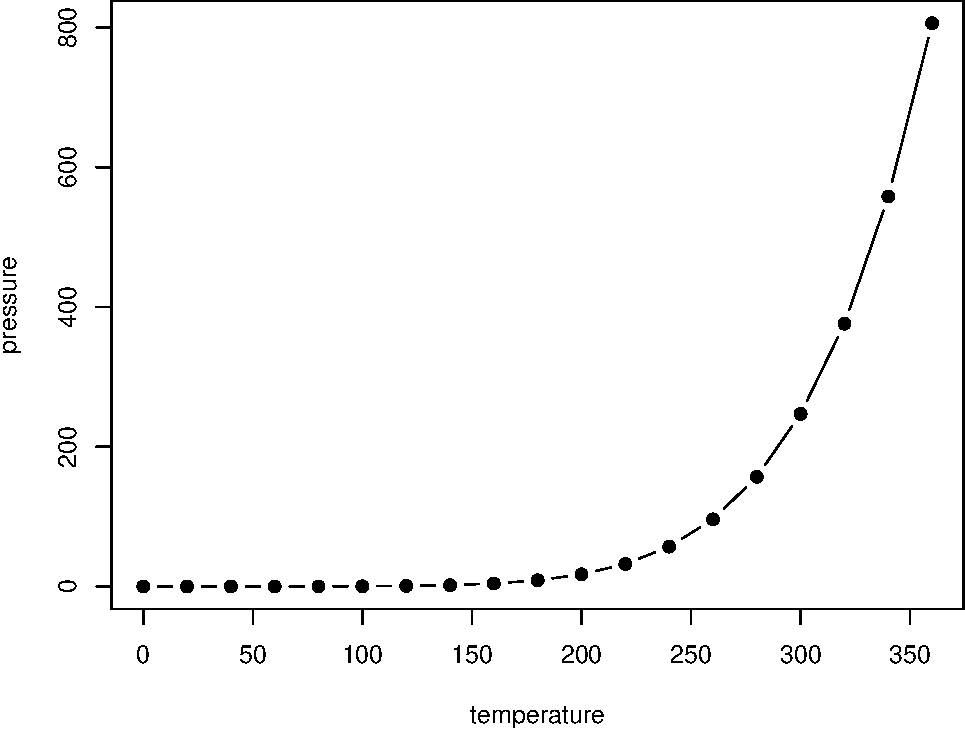
\includegraphics[width=0.8\linewidth]{_main_files/figure-latex/nice-fig-1} 

}

\caption{Here is horrible figure! Note the variable names in the axis labels. You must not do this in your dissertation. Pleases also remember the Caption Test from the EDA with R notes.}\label{fig:nice-fig}
\end{figure}

Reference a figure by its code chunk label with the \texttt{fig:} prefix, e.g., see Figure \ref{fig:nice-fig}. Similarly, you can reference tables generated from \texttt{knitr::kable()}, e.g., see Table \ref{tab:nice-tab}.

\begin{table}

\caption{\label{tab:nice-tab}Here is a table. Note the variable names in the column headings. You must not do this in your dissertation. Please also remember the Caption Test from the EDA with R lelcture notes; it is as relevant for tables as for plots.}
\centering
\begin{tabular}[t]{rrrrl}
\toprule
Sepal.Length & Sepal.Width & Petal.Length & Petal.Width & Species\\
\midrule
5.1 & 3.5 & 1.4 & 0.2 & setosa\\
4.9 & 3.0 & 1.4 & 0.2 & setosa\\
4.7 & 3.2 & 1.3 & 0.2 & setosa\\
4.6 & 3.1 & 1.5 & 0.2 & setosa\\
5.0 & 3.6 & 1.4 & 0.2 & setosa\\
\bottomrule
\end{tabular}
\end{table}

Here is an example of importing a figure, which is done inside a code chunk. Use the command \texttt{knitr::include\_graphics()} to import the figure, but use code chunk options as normal for the caption, sizing etc. You can label and refer to the figure as shown previously: see Figure \ref{fig:Rwalk}.

\begin{figure}[H]

{\centering 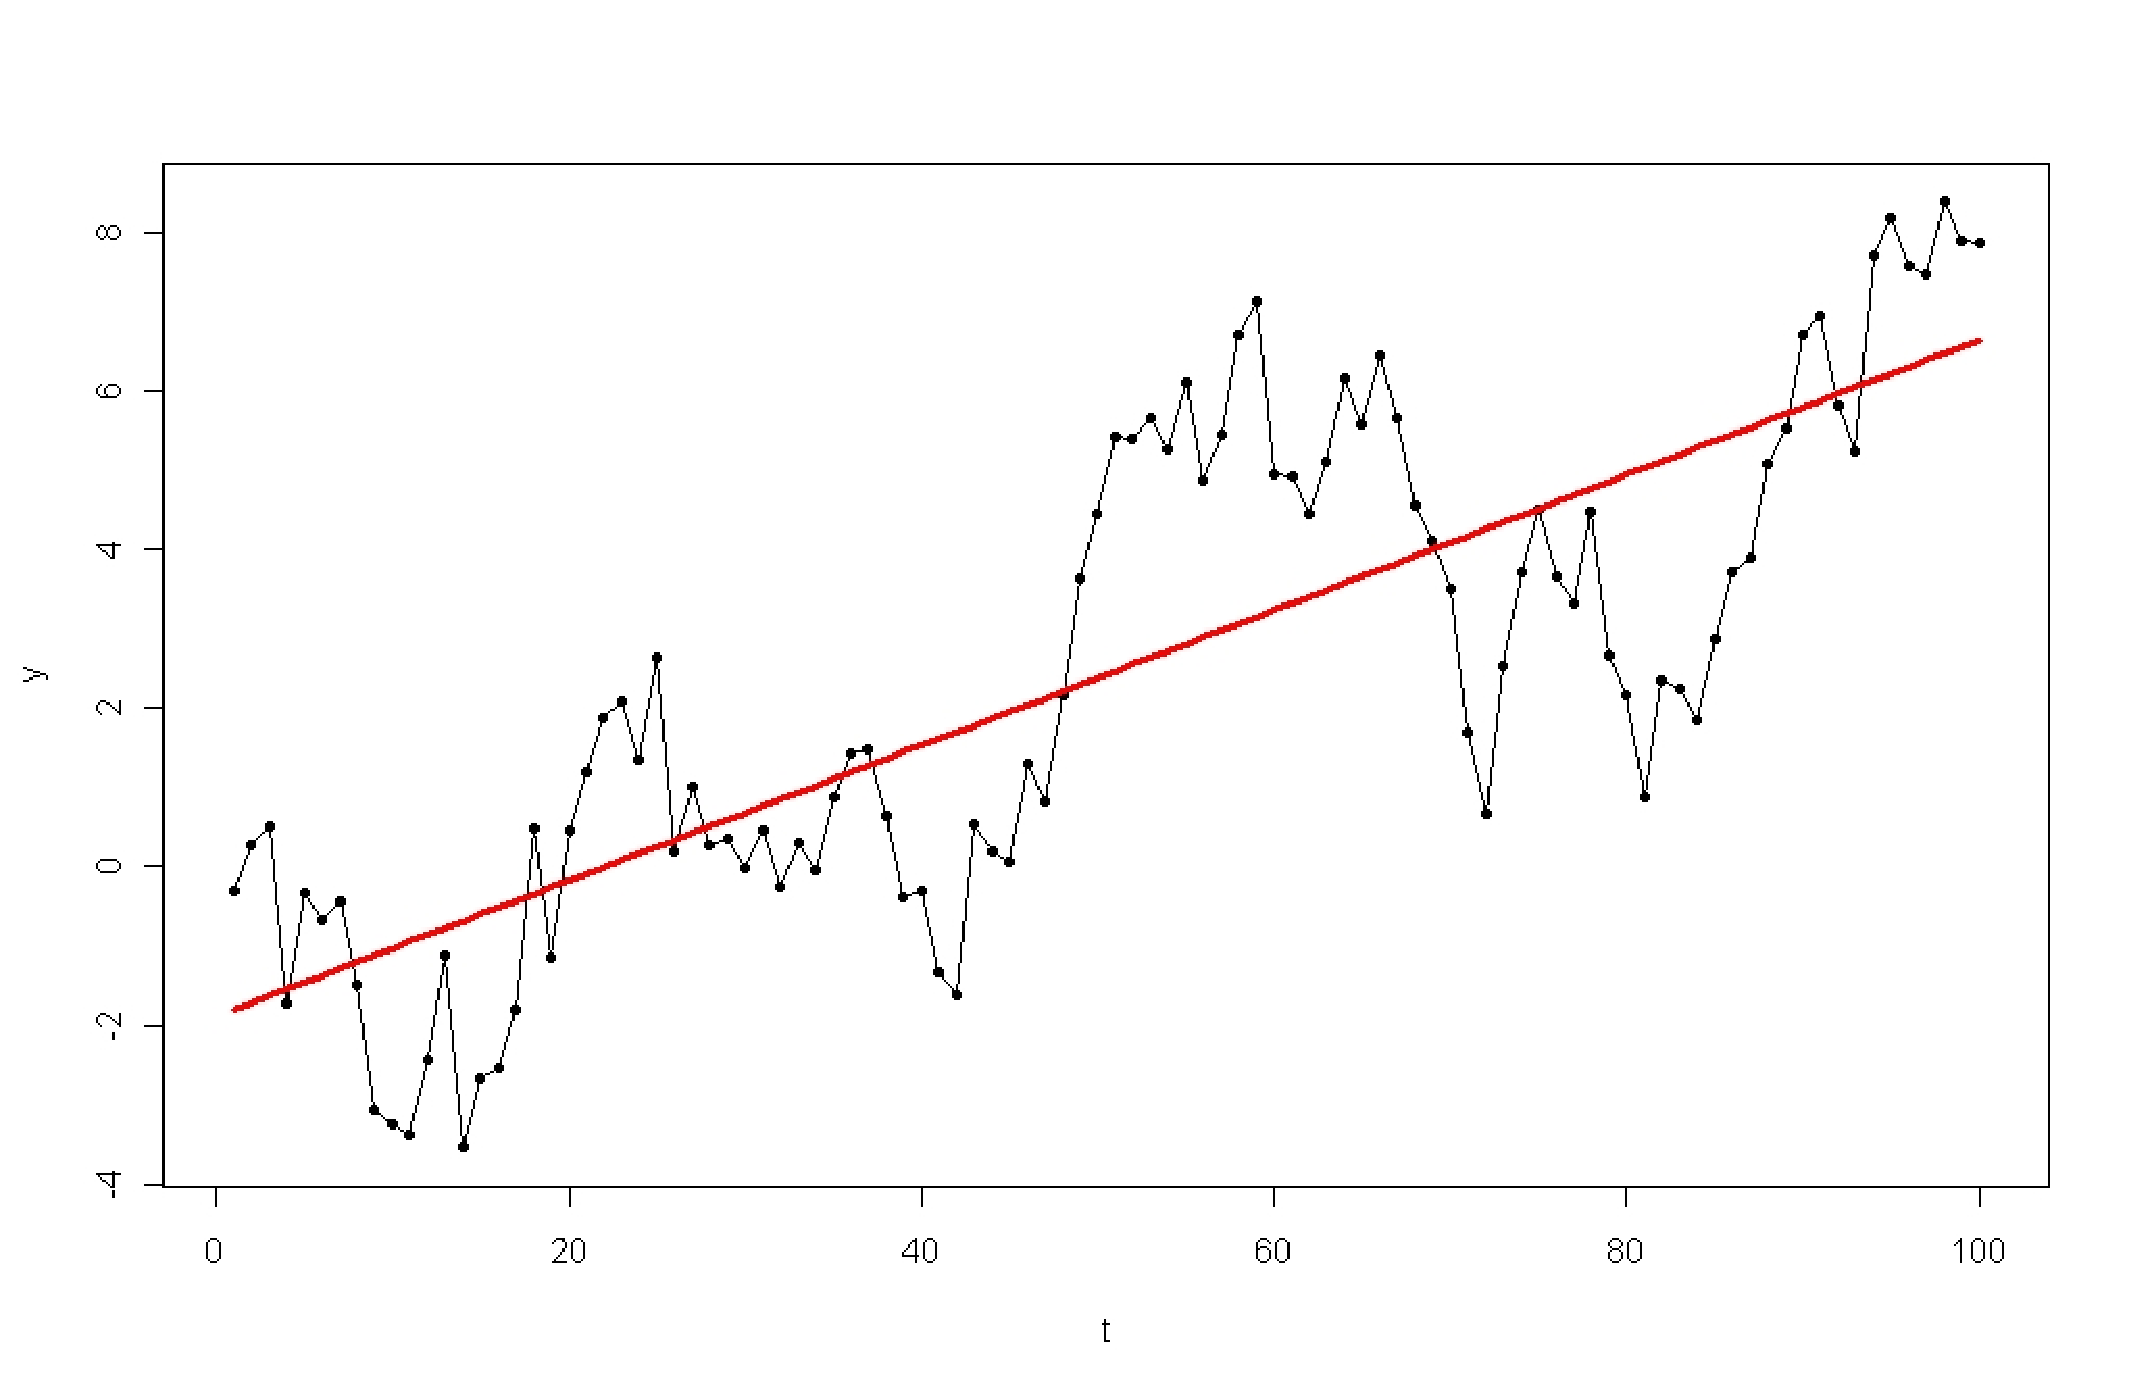
\includegraphics[width=0.8\linewidth]{figures/Rwalk} 

}

\caption{Here is another horrible figure! Again, note the variable names in the axis labels. You must not do this in your dissertation. }\label{fig:Rwalk}
\end{figure}

\hypertarget{appendix-appendix}{%
\appendix}


\hypertarget{review-of-probability-calculus}{%
\chapter{Review of probability calculus}\label{review-of-probability-calculus}}

Use appendicies only for material that is directly relevant to the contents of your dissertation and is referenced from within it. Never use it for code or for things that you found interesting, but did not in the end use for your own work.

\hypertarget{functions-of-random-variables}{%
\section{Functions of random variables}\label{functions-of-random-variables}}

\hypertarget{schwarz-inequality}{%
\section{Schwarz Inequality}\label{schwarz-inequality}}

\hypertarget{some-technical-proofs}{%
\chapter{Some technical proofs}\label{some-technical-proofs}}

\hypertarget{proof-1}{%
\section{Proof 1}\label{proof-1}}

\hypertarget{research-ethics-approval}{%
\chapter{Research Ethics Approval}\label{research-ethics-approval}}

The last appendix of your dissertation must contain evidence that you complied with the University of Sheffield research ethics approval process. Like all other appendices, it should be cross-referenced from the main text of the dissertation so that readers are alerted to its presence. The appendix should start with a paragraph of text, in your own words, that summarises the approval process as it applied to your dissertation. Here is an example to get you started.

The research ethics approval process for the work described in this dissertation was completed in March 2019, before any work using data commenced. Due to the use of data arising from \{summarise the data collection process here\}, formal research ethics approval was deemed to be necessary and, when submitted, the application was allocated reference number: 000094. Formal approval is evidenced here by inclusion of the final approval letter in Figure \ref{fig:ethicsapprov}.

\newpage

\begin{figure}[H]

{\centering 
\includegraphics[width=1\linewidth]{figures/ApprovalLetterCrop} 

}

\caption{The research ethics approval letter provided for the work outlined in this dissertation, following compliance with the University of Sheffield offical research ethics processes.}\label{fig:ethicsapprov}
\end{figure}

\hypertarget{references}{%
\chapter*{References}\label{references}}
\addcontentsline{toc}{chapter}{References}

\hypertarget{refs}{}
\begin{cslreferences}
\leavevmode\hypertarget{ref-dellas}{}%
Dellaportas, P., J. J. Foster, and I. Ntzoufras. 2000. ``Bayesian Variable Selection Using the Gibbs Sampling.'' In \emph{Generalized Linear Models: A Bayesian Perspective}, edited by S. K. Ghosh D. K. Dey and B. K. Mallick, 273--86. New York: Marcel Dekker.

\leavevmode\hypertarget{ref-Fristedt}{}%
Fristedt, B. E., and L. F. Gray. 1996. \emph{A Modern Approach to Probability Theory}. Birkhäuser Boston.

\leavevmode\hypertarget{ref-lambert}{}%
Lambert, P. C., A. J. Sutton, P. R. Burton, K. R. Abrams, and D. R. Jones. 2005. ``How Vague Is Vague? A Simulation Study of the Impact of the Use of Vague Prior Distributions in MCMC Using WinBUGS.'' \emph{Statistics in Medicine} 24: 2401--28.

\leavevmode\hypertarget{ref-Williams}{}%
Williams, D. 1991. \emph{Probability with Martingales}. Cambridge University Press.
\end{cslreferences}

\end{document}
